\documentclass[margin = 10pt]{standalone} 
\usepackage{tikz}
\usepackage{pgfplots}
\pgfplotsset{compat = 1.18}

\begin{document}
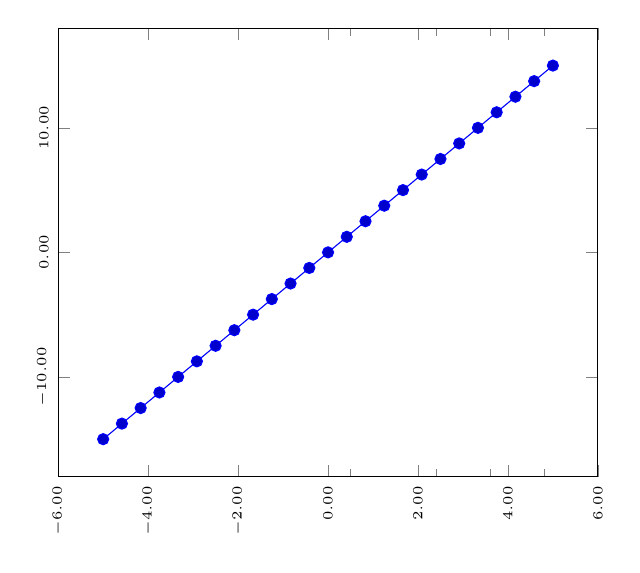
\begin{tikzpicture}[remember picture]
\begin{axis}[
    % 
    % 刻度数值
    % 空
    % xtick= \empty,
    % 自动分配
    xtick= {},
    % 从数据中加载
    % xtick= data,
    % 特殊指定
    % xtick= {1,2,3,4},
    % 
    % 子刻度
    % minor xtick={},
    minor xtick={0.5,2.4,3.6,4.8},
    % 
    % scaled ticks = real:10,
    % 
    % 样式设置
    % xticklabel style ={},
    % yticklabel style ={}, 
    ticklabel style = {
        /pgf/number format/fixed zerofill,
        /pgf/number format/precision=2,
        font = \tiny,
        rotate = 90
        },
    ]
    
\addplot   {x*3};
\end{axis}
\end{tikzpicture}
\end{document}